\chapter{Implementation Detail}

\section{Development Environment}

无论是手表端的还是服务端,都存在框架依赖,因此环境搭建不可避免。在本项目中,服务端使用 NodeJS 进行编码,限于篇幅,对 NodeJS 相关的基本环境,如 Node 本体,NPM 包管理等常见工具的配置在文中略去,这里主要介绍运行本平台最重要第三方 Leap Motion 环境;而在手表端中,虽然我们不依赖其他第三方框架,但由于 watchOS 自身的限制\cite{WatchConnectivity:2016} 在 watchOS 2 中我们需要使用 WatchConnectivity 框架与 iOS 应用本体进行数据通信。
由于 iOS 系统本身限制(iOS 9及以上)强制要求应用必须与 HTTPS 服务器进行通信,因此这里介绍在 iOS 9 中与 HTTP 服务器通信的配置方法。

\subsection{Configuration of Local LeapMotion}

LeapMotion 提供了在 Mac OS X 中的开发环境,并且提供了各种不同的开发语言,根据上文的讨论,我们需要在服务端配置 LeapMotion 本体以及 LeapJS。

\textbf{1. Installation}

首先,在应用程序中引入 Leap SDK 需要在相应桌面端安装 LeapMotion 宿主程序,进而才能使用 LeapMotion 相关的 API。

其次,在 Node App 的 package.json 中添加 LeapJS 依赖:
\begin{lstlisting}[frame=trBL,frameround=fttt,rulesepcolor=\color{White},numbers=none]
"dependencies": {
    "leapjs": "^0.6.4"
}
\end{lstlisting}
再使用 npm install 安装 LeapJS。

\textbf{2. Configuration}

受到 LeapMotion 自身的限制\cite{Leap:2016},WebSocket 服务并非默认的向非本地访问开放,因此需要将 Leap 配置启用非本地客户端连接。

这需要对 LeapMotion 的配置文件进行修改。在修改配置之前,需要关闭 LeapMotion 的相关服务。在 Mac 中,使用下面的命令关闭 LeapMotion 的守护进程:
\begin{lstlisting}[frame=trBL,frameround=fttt,rulesepcolor=\color{White},numbers=none]
sudo launchctl unload /Library/LaunchDaemons/com.leapmotion.leapd.plist
\end{lstlisting}

接下来我们需要修改 LeapMotion 的配置文件,根据 LeapMotion 的官方文档显示,Leap 包含两个不同的配置,其中控制面板配置的优先级最高,因此我们需要下面这个目录下:
\begin{lstlisting}[frame=trBL,frameround=fttt,rulesepcolor=\color{White},numbers=none]
$HOME/Library/Application\ Support/Leap\ Motion
\end{lstlisting}

找到 config.json 的修改配置,编辑 config.json 文件,并在 configuration 字段中的任意位置添加一条:
\begin{lstlisting}[frame=trBL,frameround=fttt,rulesepcolor=\color{White},numbers=none]
"websockets_allow_remote": true
\end{lstlisting}

最终得到:

\begin{lstlisting}[frame=trBL,frameround=fttt,rulesepcolor=\color{White},numbers=none]
"configuration": {
    "websockets_allow_remote": true,
    "background_app_mode": 2,
    "images_mode": 2,
    "interaction_box_auto": true,
    "power_saving_adapter": true,
    "robust_mode_enabled": false,
    "tracking_tool_enabled": true
}
\end{lstlisting}

保存退出,重新启动 LeapMotion 服务,便完成了 LeapMotion 的相关配置:

\begin{lstlisting}[frame=trBL,frameround=fttt,rulesepcolor=\color{White},numbers=none]
sudo launchctl load /Library/LaunchDaemons/com.leapmotion.leapd.plist
\end{lstlisting}

\subsection{Configureation of watchOS Networking}

从 iOS 9 开始, iOS 对网络访问引入了 App Transport Security (ATS) 特性,这使得在默认状态下 iOS 应用无法发起非安全的网络请求(如 HTTP)。
需要进行下列两个步骤配置项目,结果如图\ref{fig:config}所示:

\begin{enumerate}
    \item 在Info.plist中添加NSAppTransportSecurity类型Dictionary;
    \item 在NSAppTransportSecurity下添加NSAllowsArbitraryLoads类型Boolean,值设为YES
\end{enumerate}

\begin{figure}[H]
    \kaishu
    \centering
    \includegraphics[width=0.4\textwidth]{figures/config}
    \caption{\kaishu 配置客户端 info.plist 文件}
    \label{fig:config}
\end{figure}

\section{Server-Side Core}

实现一个端口为 10086 的 HTTP 服务器是第一步,如代码\ref{lst:http}。
\begin{lstlisting}[
    language={JavaScript},
    caption={\kaishu 在 10086 端口创建 HTTP 服务器},
    label={lst:http}
]
var http = require('http');
function handler (req, res) {
    res.writeHead(200);
}
http.createServer(handler).listen(10086);
console.log("Server running at http://locoalhost:10086")
\end{lstlisting}

下面我们来关注服务端中对 LeapMotion 手势的关键处理。

\subsection{Tap and Force Touch Recognition}

LeapMotion 软件本身会对所识别手部进行重新建模,并提供其骨骼模型的全部数据,因此也包括对手指位置。
而对于手指捏合的识别,可以转化为对两只手指指尖位置的判断,故可对除拇指外的其他四根手指中进行遍历,如代码\ref{lst:pincher} 所示。

\begin{lstlisting}[
    language={JavaScript},
    caption={\kaishu 手指点按识别},
    label={lst:pincher}
]
pinchIndex = function findPinchingFinger(hand, closest) {
    var pincher;
    for(var f = 1; f < 5; f++) {
        current = hand.fingers[f];
        distance = leap.vec3.distance(
            hand.thumb.tipPosition,
            current.tipPosition
        );
        if(current != hand.thumb && distance < closest) {
            closest = distance;
            pincher = current;
        }
    }
    return pincher;
}
\end{lstlisting}

对于 Force Touch 的模拟在\ref{sub:force-touch-simu}一节中已经详细描述过方法,其核心实现如代码\ref{lst:ft-simu}所示。
\begin{lstlisting}[
    language={JavaScript},
    caption={\kaishu Force Touch 仿真},
    label={lst:ft-simu}
]
forceValue = function(……){
    ……【待补充】
}
\end{lstlisting}

\subsection{Two Fingers Slipe}

对于双指之间滑动的识别看似困难,但实际上我们可以将其转化为两指之间的捏合度。其实 LeapMotion 本身提供了对拇指和食指捏合度参数,但由于其结果为一般情况下的捏合度,即在任何收拾下都存在捏合度,而对于我们来说需要控制交互,构建双指滑动的触发事件,因此我们有必要重新实现这个功能。

\begin{figure}[H]
\kaishu
\centering
\subfigure[滑动前]{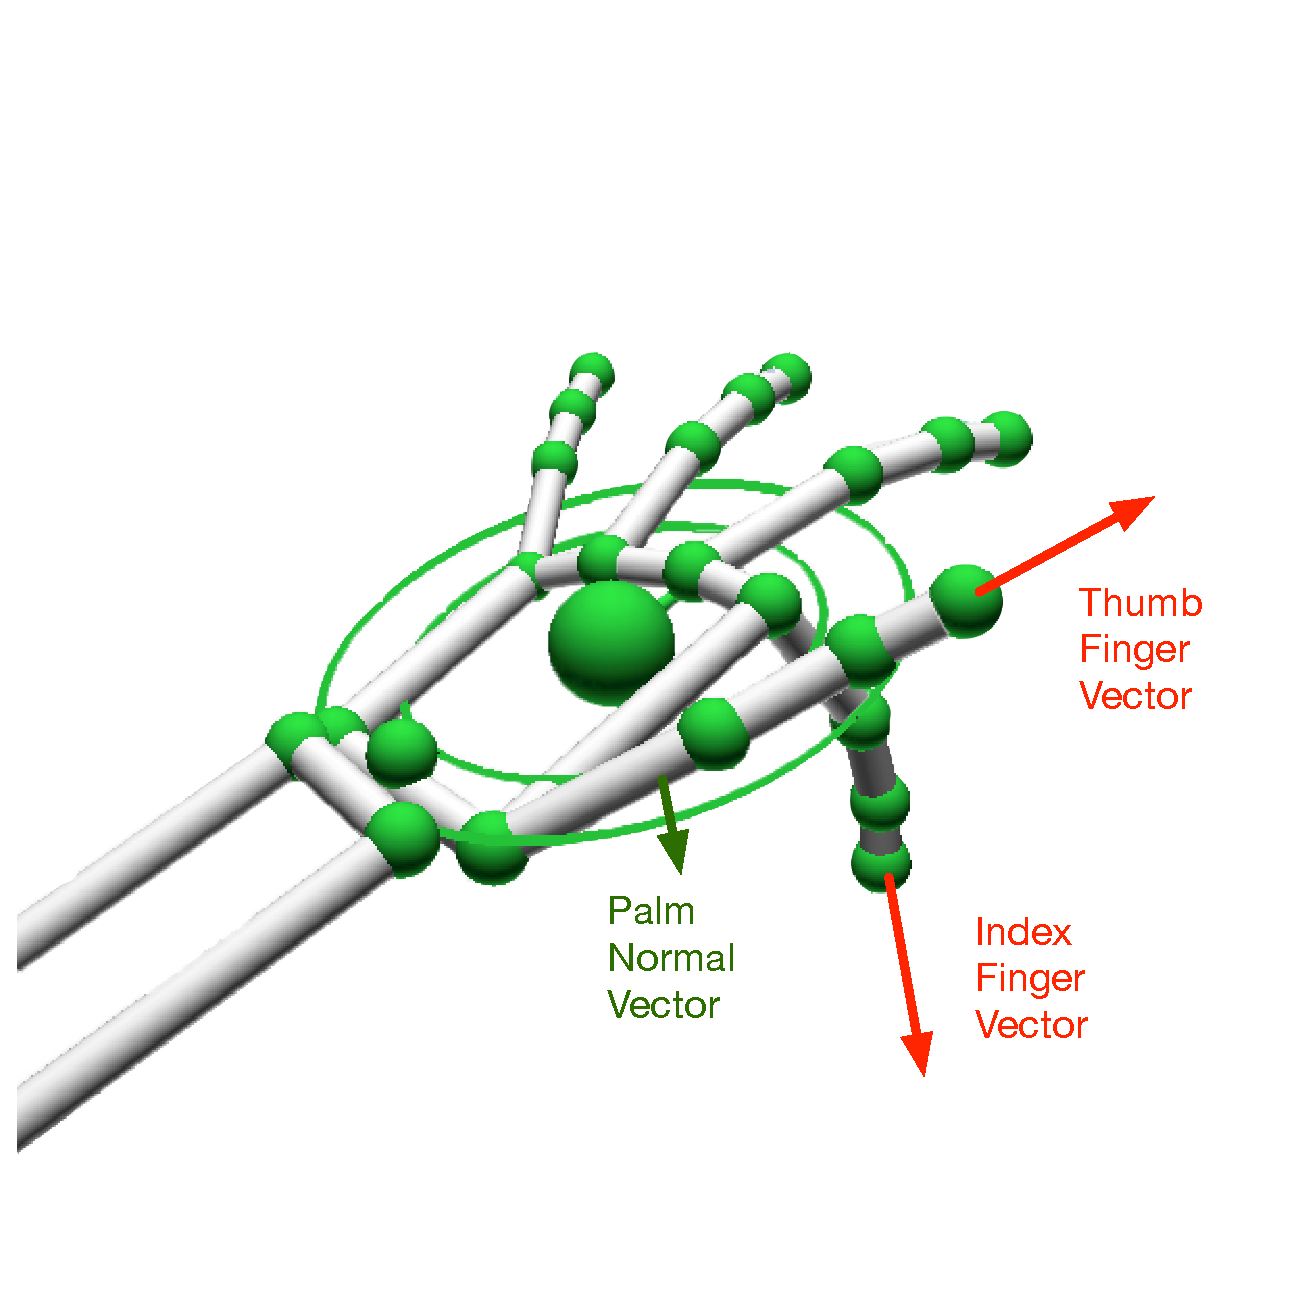
\includegraphics[width=0.35\textwidth]{figures/pinch-start}\label{fig: pinch-start}}
\subfigure[滑动后]{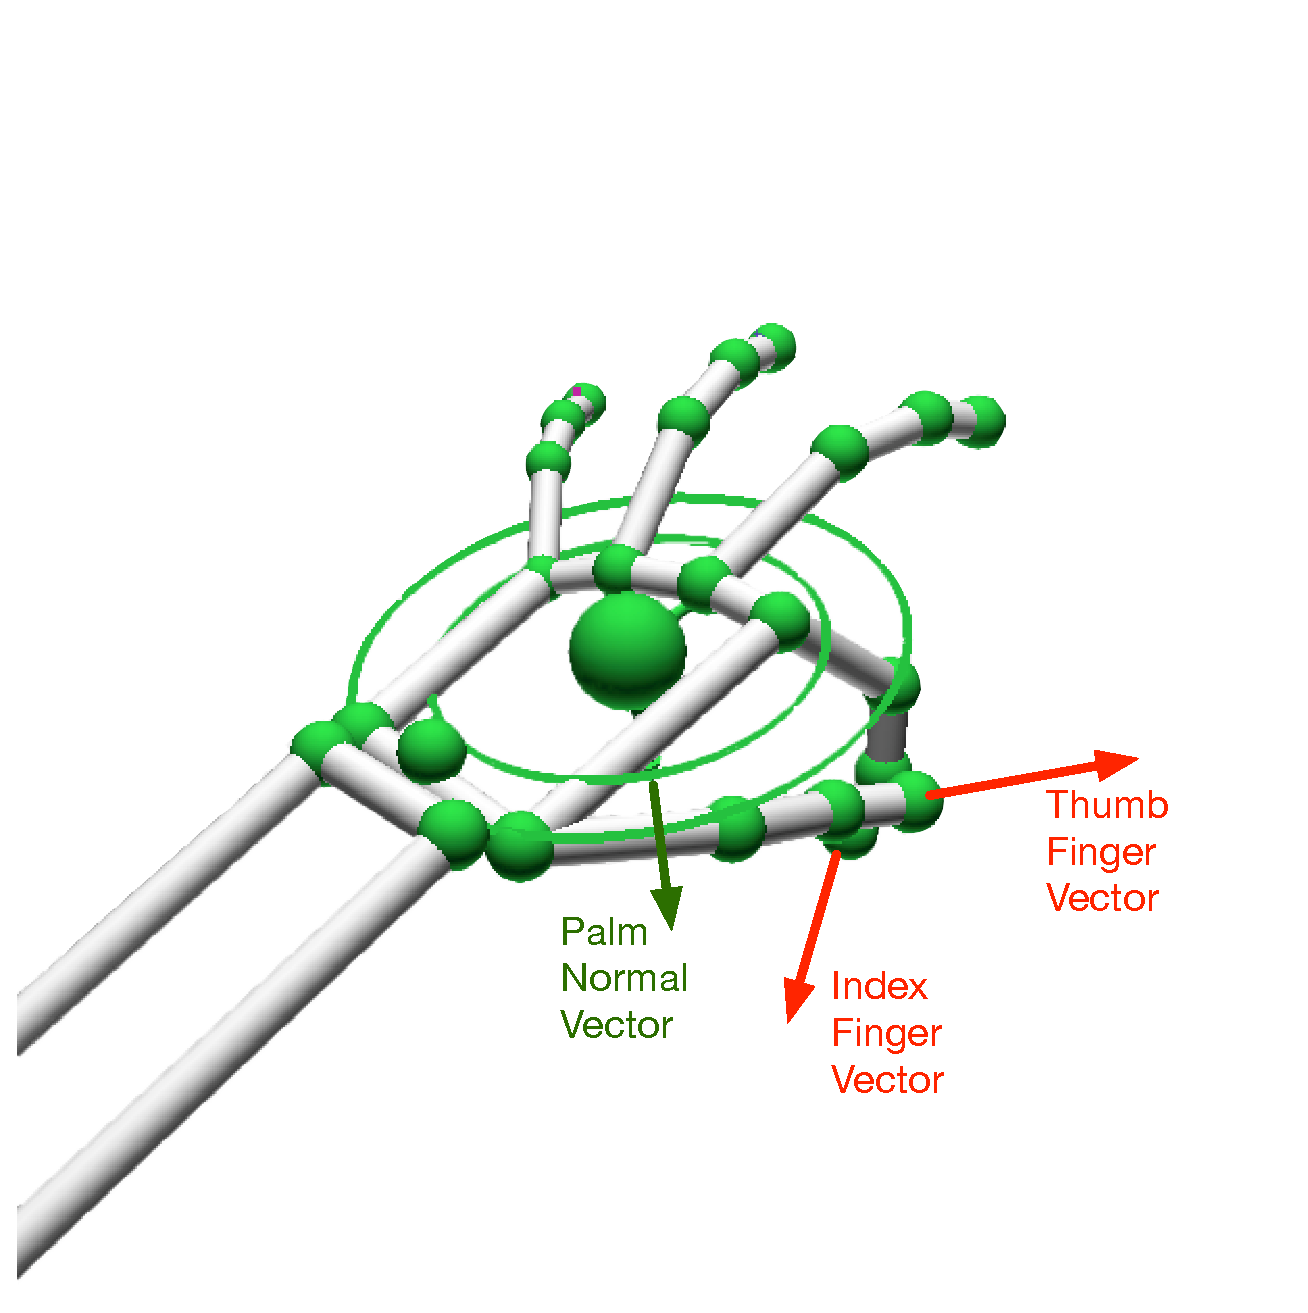
\includegraphics[width=0.35\textwidth]{figures/pinch-end}\label{fig:pinch-end}}
\caption{\textbf{双指滑动}:双指滑动可以通过手指和手掌的指向向量设计触发事件}
\label{fig:pinch}
\end{figure}

双指滑动手势如图\ref{fig:pinch}所示,当手呈现如图\ref{fig: pinch-start}所示手势时,食指的方向向量和手掌的法向量几乎平行,拇指的方向向量与手掌的法向量几乎垂直,故我们可以利用这个特点设计手势的触发事件。如代码\ref{lst:swipe}:

\begin{lstlisting}[
    language={JavaScript},
    caption={\kaishu 手指点按识别},
    label={lst:swipe}
]
pinchStrength = function findPinchStrength(hand, closest) {
    ……【待补充】
}
\end{lstlisting}

\subsection{Full Fingers Grab}

五指的合并不需要重新实现,LeapMotion 本身就提供了握拳程度的参数 grabStrength,我们可以直接从 Frame 对象中获取,如代码\ref{lst:grab}所示。

\begin{lstlisting}[
    language={JavaScript},
    caption={\kaishu 五指合并识别},
    label={lst:grab}
]
grabStrength = function getGrabStength(frame) {
    return frame.hands[0].grabStrength;
}
\end{lstlisting}

\section{Client-Side Core}

手表端编码的两个重要关键就是通信层和视图控制层的编码,通信层又包含 iOS 端和服务端之间通信以及 iOS 端和 watchOS 端间通信,我们使用 Swift \footnote{本文写成时的 Swift 版本为 2.2。}来完成相关编码\cite{swift2015, swiftoc2015}。

\subsection{View Controller Core}

【待补充】

\subsection{Communication Layer Core}

与服务端的通信通过 URL 请求服务端的手势数据,其结果为 JSON 格式数据。在代码\ref{lst:connectserver}中, completeFlag 保证了向服务器请求对象时仅在上一次请求完成后才能进行,而 Gesture 类的构造函数通过从 URL 中解析来的 JSON 数据字典构造 Gesture 对象模型。

\begin{lstlisting}[
    language={Swift},
    caption={\kaishu iOS 端与服务端通信},
    label={lst:connectserver}
]
func connectServer() {
    // member variable
    if completeFlag == 0 {
        return
    }
    task = session.dataTaskWithURL(url, completionHandler: { (data, res, error) -> Void in
        if let e = error {
            print("dataTaskWithURL fail: \(e.debugDescription)")
            return
        }
        if let d = data {
            print("\(NSString(data: d, encoding: NSUTF8StringEncoding))")

            if let jsonObj = try? NSJSONSerialization.JSONObjectWithData(d, options: NSJSONReadingOptions.AllowFragments) as? NSDictionary {
               self.Gesture = Gesture(fromDictionary: jsonObj!)
            }
            self.completeFlag = 1

        }
    })
    task!.resume()
}
\end{lstlisting}

在 iOS 端和 watchOS 端之间通信需要利用 WatchConnectivity 框架,代码包含 iOS 端发送以及 watchOS 端接受,如代码\ref{lst:ios-watchos} 和 \ref{lst:watchos-ios}所示。

\begin{lstlisting}[
    language={Swift},
    caption={\kaishu \textbf{iOS 端与 watchOS 通信}:发送},
    label={lst:ios-watchos}
]
func updateMessage() {
    if WCSession.defaultSession().reachable {
        let content:[String:String] = ["x":PinchFinger.text!, "y":PinchStrength.text!, "z":GrabStrength.text!]
        let message = ["up": content]
        WCSession.defaultSession().sendMessage(
            message, replyHandler: { (replyMessage) -> Void in
                print("send success..")
            }) { (error) -> Void in
                print(error)
        }
    }
}
\end{lstlisting}
\begin{lstlisting}[
    language={Swift},
    caption={\kaishu \textbf{watchOS 端与 iOS 通信}:接收},
    label={lst:watchos-ios}
]
extension InterfaceController: WCSessionDelegate {
    func session(session: WCSession, didReceiveMessage message: [String : AnyObject]) {
        guard message["up"] as? [String:String] != nil else {return}
        let contents = message["up"] as! [String : String]
        self.interaction(contents)
    }
}
\end{lstlisting}
